\def\pathToRoot{../../}
\def\DLbook{https://www.deeplearningbook.org/}
\def\LAchapter{https://www.deeplearningbook.org/contents/linear_algebra.html}
\def\post{https://towardsdatascience.com/linear-algebra-for-deep-learning-f21d7e7d7f23}

\documentclass[a4paper, 12pt]{article}

\usepackage[utf8]{inputenc}
\usepackage{ifthen}
\usepackage{xparse}
\usepackage{scrextend}
\usepackage{setspace}
\usepackage{verbatim}
\usepackage{color}
\usepackage[inline]{enumitem}
\usepackage[colorlinks=true, linkcolor=black, citecolor=black]{hyperref}

\usepackage{tikz}
\usepackage{pgfplots}
\usepackage{bbold}
\usepackage{listings}

\usepackage{subcaption}

\usepackage{amsmath}
\usepackage{amssymb}
\usepackage{latexsym}
\usepackage{hyperref}


%% added by Sangeet
\usepackage{csquotes}
\usepackage{booktabs}
\usepackage{amsmath}
\usepackage{mathtools}% http://ctan.org/pkg/mathtools
\usepackage{caption}
\captionsetup{width=.75\textwidth}
\usepackage[usestackEOL]{stackengine}
\usepackage{float}

\usepackage{tikz}
\usetikzlibrary{shapes.geometric,arrows,positioning,fit}
\usetikzlibrary{shapes,calc,arrows}
\usepackage{natbib}
\usepackage{graphicx}
\usepackage{hyperref}
\usepackage{url}
\usepackage[super]{nth}
\usepackage{xcolor}
% \usepackage{authblk}
% \usepackage{microtype}

        
\definecolor{gray}{rgb}{0.2,0.2,0.2}

\pagenumbering{arabic}

\input{HW1/uebungsheader}
\def\issolution{}


\begin{document}

% {Sheet number}{headline}{deadline}
\exercisehead{1}{Linear Algebra Basics}{17.11.2020, 23:59}

\section*{Instructions}

A good understanding of linear algebra is essential for understanding and working with many machine learning algorithms, especially deep learning algorithms.
The purpose of the following exercises is to create the base for understanding concepts and algorithms introduced in the following lectures.

The exercises are based on the \href{\post}{\textit{Basic Linear Algebra for Deep Learning} post} by Niklas Donges and the \href{\LAchapter}{\textit{Linear Algebra} chapter} in the \href{\DLbook}{\textit{Deep Learning} book} by Ian Goodfellow, Yoshua Bengio and Aaron Courville.

\section*{Exercises}

\begin{exercise}[Mathematical objects][1]
 Consulting \href{\post}{Niklas's post} or \href{\LAchapter}{Deep Learning book}, give short definitions and your own examples.
 
 Note the conventional way to define different mathematical objects (you can find them in the \href{\LAchapter}{DL book}), e.g. we write scalars in italics and usually give them lowercase variable names.
 Throughout all the assignments (and of course outside of this course) stick to the conventional way of writing scalars, vectors etc\footnote{See how to make letters bold in LaTex math mode  \href{https://tex.stackexchange.com/questions/14395/bold-italic-vectors}{here}.}.
 
 \begin{enumerate}
     \item scalar
     \item vector
     \item matrix
     \item tensor
 \end{enumerate}

\end{exercise}


\begin{solution}
   % write the solution here
   \color{blue}
   \begin{enumerate}
       \item A \textbf{scalar} is just a single number. We write scalars in italics and usually give them lowercase variable names.
        \math
        s \in R , s = 0.2
        \endmath

        \item A \textbf{vector} is an ordered array of numbers. Typically we give vectors lowercase names in bold typeface. The elements of the vector are identified by writing its name in italic typeface.
        \math
            \textbf{x} = \begin{bmatrix}
            x_1 & x_2 & x_3
            \end{bmatrix}
        \endmath

        \item A \textbf{matrix} is a 2-D array of numbers, where each element is identified by indices instead of just one. We usually give matrices uppercase variable names with bold typeface, such as \textbf{A}. The elements of the matrix are identified by writing its name in italic typeface.

        \math
            \textbf{A} = \begin{bmatrix}
            x_1 & x_2 & x_3 \\
            x_4 & x_5 & x_6 \\
            x_7 & x_8 & x_9
            \end{bmatrix}
        \endmath


        \item A \textbf{tensor} is an array of numbers, arranged on a regular grid, with a variable number of axes. A tensor has three indices, where the first one points to the row, the second to the column and the third one to the axis. We denote a tensor named “A” with this typeface: A.
        
        We identify the element of A at coordinates $ (i,j,k)$  by writing  $ \textbf{A}_{i,j,k}$.

 \end{enumerate}
\end{solution}

\begin{exercise}[Vectors in machine learning][2]

In machine learning we deal with data in multidimensional space.
Each data point is characterised by a number of features: for example, a lecture can be characterised by the number of CoLi students, CS students and students from other departments (i.e. 3 features).

\begin{figure}[h]
    \centering
    \includegraphics[width=.8\textwidth]{figures/vectors.png}
    \caption{Different vector representations. Note: those are not representations of the same vector}
    \label{fig:vector_representations}
\end{figure}

\begin{enumerate}
\item Create your own data set of \textbf{three} data points where each data point is described by \textbf{two} features.
Report:
    \begin{enumerate}
        \item what are the data points in your data set (e.g. lectures);
        \item what are the features of the data points (e.g. number of CoLi students).
    \end{enumerate}

\item Represent the data set in physical space (as in Figure \ref{fig:vector_representations}).
Label the axes according to the features you defined.

\item Represent the data in form of vectors $\vect{x_1}, \vect{x_2}, \vect{x_3}$.

\item Represent the data in form of a matrix $\vect{X} \in \mathbb{R}^{n\times m}$, where $n$ is the number of data points and $m$ is the number of features.

\end{enumerate}

\end{exercise}

\begin{solution}
   % write the solution here
   \color{blue}
   
   \begin{enumerate}
       \item This dataset comprises number of letters in the alphabet vs. number of phonemes in three languages: Arabic, Hindi and Lithuanian.
       
       \begin{enumerate}
            \item Data points - Arabic, Hindi, Lithuanian.
           \item Features of the data points - number of letters in alphabet, number of phonemes.
       \end{enumerate}
       
       \item 
    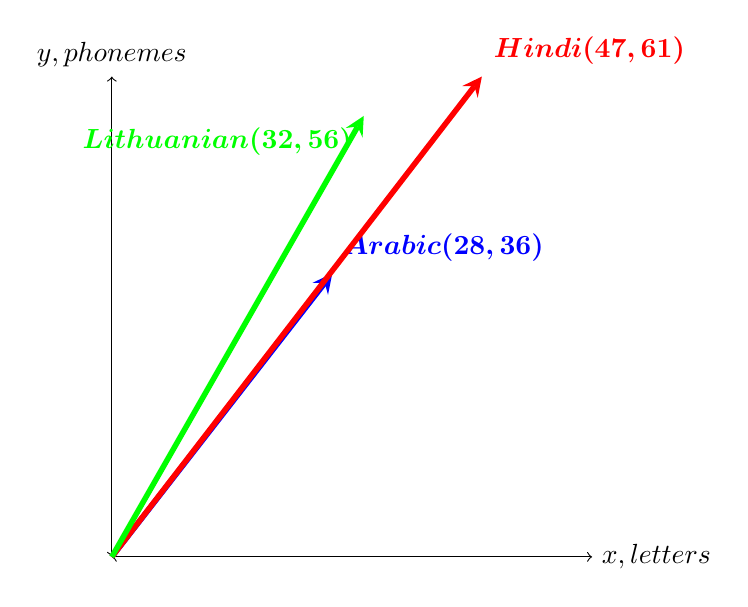
\begin{tikzpicture}
  \draw[<->] (0,0)--(6.1,0) node[right]{$x, letters$};
  \draw[<->] (0,0)--(0,6.1) node[above]{$y, phonemes$};
  \draw[line width=2pt,blue,-stealth](0,0)--(2.8,3.6) node[anchor=south west]{$\boldsymbol{Arabic(28,36)}$};
  \draw[line width=2pt,red,-stealth](0,0)--(4.7,6.1) node[anchor=south west]{$\boldsymbol{Hindi(47,61)}$};
  \draw[line width=2pt,green,-stealth](0,0)--(3.2,5.6) node[anchor=north east]{$\boldsymbol{Lithuanian(32,56)}$};
\end{tikzpicture}

       \item
       Arabic:\\
     $$\vect{x1} = \begin{bmatrix} \texttt{28} \\  \texttt{36} \end{bmatrix} $$ \\
     Hindi:\\
     $$\vect{x2} = \begin{bmatrix} \texttt{47} \\  \texttt{61} \end{bmatrix} $$ \\
     Lithuanian:\\
     $$\vect{x3} = \begin{bmatrix} \texttt{32} \\  \texttt{56} \end{bmatrix} $$
     
       \item
    $\vect{X} \in \mathbb{R}^{n\times m}$\\
    $\vect{X} = \begin{bmatrix} 28 & 47 & 32 \\ 36 & 61 & 56 \end{bmatrix}$
   \end{enumerate}
\end{solution}

\begin{exercise}[Operations on vectors and matrices][2.5]

We can perform mathematical operations such as addition, subtraction, multiplication on vectors, matrices and scalars.
Carefully read the \textit{Computational rules} part of the \href{\post}{post\footnote{Pay attention to the dimensions and use the cheat sheets provided by Niklas.}} and perform the following exercises.
If the computation is impossible, write \textit{impossible} and argue why.

\begin{enumerate}
    \item $\begin{bmatrix} 3 & 4 & 1 \\ 0 & 2 & 3 \end{bmatrix} \div 2 = $
    \item $\begin{bmatrix} 3 & 4 & 1 \\ 0 & 2 & 3 \end{bmatrix} \ast \begin{bmatrix} 2 \\ 1 \\ 5  \end{bmatrix} = $
    \item $\begin{bmatrix} 3 & 4 & 1 \\ 0 & 2 & 3 \end{bmatrix} - \begin{bmatrix} -1 & 2 & 10 \\ 3 & -6 & 3 \end{bmatrix} = $
    \item $\begin{bmatrix} 3 & 4 & 1 \\ 0 & 2 & 3 \end{bmatrix} \ast \begin{bmatrix} 0 & 2 \\ 1 & -2 \\ 4 & 0 \end{bmatrix} = $
    \item $\begin{bmatrix} 3 & 4 & 1 \\ 0 & 2 & 3 \end{bmatrix} \ast \begin{bmatrix} 10 & 5 \\ 0 & 2 \end{bmatrix} = $
\end{enumerate}

If you are interested in the physical meaning of vectors, matrices and operations on them, watch videos from the \href{https://www.youtube.com/playlist?list=PLZHQObOWTQDPD3MizzM2xVFitgF8hE_ab}{Linear Algebra} series by \href{https://www.youtube.com/channel/UCYO_jab_esuFRV4b17AJtAw}{3Blue1Brown}.

\end{exercise}

\begin{solution}
   % write the solution here
   \color{blue}
    \begin{enumerate}
    \item   \math
                \begin{bmatrix}
                    1.5 & 2 & 0.5 \\
                    0 & 1 & 1.5
                \end{bmatrix}
            \endmath
        
    \item   \math
                \begin{bmatrix}
                    15\\
                    17
                \end{bmatrix}
            \endmath
        
        
    \item   \math
                \begin{bmatrix}
                    4 & 2 & -9 \\
                    -3 & 8 & 0
                \end{bmatrix}
         \endmath
        
    \item   \math
                \begin{bmatrix}
                    8 & -2 \\
                    14 & -4
                \end{bmatrix}
            \endmath

        
        \item Impossible. As number of columns in first matrix doesn't match number of rows in the second one.
                 
    \end{enumerate}
   
\end{solution}

\begin{exercise}[Multiplication properties and types of matrices][3.5]

Read chapters \textit{2.2 Multiplying Matrices and Vectors} and \textit{2.3 Identity and Inverse Matrices} of the \href{https://www.deeplearningbook.org/contents/linear_algebra.html}{DL book} or corresponding parts of the \href{https://towardsdatascience.com/linear-algebra-for-deep-learning-f21d7e7d7f23}{Niklas's post}

On the internet, find the following definitions and write them down:
\begin{enumerate}
    \item symmetric matrix
    \item orthogonal matrix
    \item unit vector
    \item orthogonal vectors
\end{enumerate}

Let $\vect{A}^{n \times n}$ be an orthogonal matrix, $\vect{B}^{m \times m}$ -- a symmetric matrix and $\vect{C}^{m \times n}$ -- a regular matrix, $\vect{I}$ -- identity matrix, and $\lambda$ - a scalar. \\
    For each expression choose its equivalent, show the intermediate steps, give the dimensions of the result. \vspace*{0.5em} \\
    $(\vect{B} \lambda \vect{I})^T\vect{C} = $ \\
    \begin{enumerate*}
        \item $\lambda \vect{CB}$ \hspace*{3em}
        \item $\vect{CB}^T  \lambda$ \hspace*{3em}
        \item $\lambda \vect{BCI}$
    \end{enumerate*}
    \vspace*{0.5em} \\
    $\vect{A}^{-1}(\vect{CA}^{-1})^T \lambda = $ \\
    \begin{enumerate*}
        \item $\lambda \vect{C}^T$ \hspace*{3em}
        \item $\lambda \vect{C}$ \hspace*{4.5em}
        \item $\vect{A}^T\vect{C}^T \lambda$
    \end{enumerate*}
    \vspace*{0.5em} \\
    $\vect{AA}^T\vect{B}^T\vect{C} = $ \\
    \begin{enumerate*}
        \item $\vect{CB}$ \hspace*{3.2em}
        \item $\vect{B}^{-1}\vect{C}$ \hspace*{3.8em}
        \item $\vect{BC}$
    \end{enumerate*}
    

\end{exercise}

\begin{solution}
   \color{blue}
   \begin{enumerate}
       \item A \textbf{symmetric matrix} is a square matrix that satisfies $ A^T = A$. The entries of a symmetric matrix are symmetric with respect to the main diagonal. If $A$ is a symmetric matrix, then for every $i$,$j$ $$ a_{ij} = a_{ji}$$

        \item An \textbf{orthogonal matrix} is a real square matrix whose columns and rows are orthogonal unit vectors. When matrix $Q$ is orthogonal, the given is true:
        $$
        Q\mathord{\cdot}Q^T = Q^T\mathord{\cdot}Q = I
        $$

        \item A \textbf{unit vector} is a vector of length 1 , and is denoted by circumflex or “hat”: $\hat{u}$ 
        \item \textbf{Orthogonal vectors} are two vectors $u$ and $v$ whose dot product- $$u\mathord{\cdot}v = 0$$
   \end{enumerate}

   \begin{enumerate}
       \item The answer is \textbf{c}.\\
        $ (B_{m \times m}\lambda I_{m \times m})^{T}C_{m \times n}$\\
        $= \lambda B_{m \times m}^{T}C_{m \times n}$ (Property used- $B^T=B$)\\
        $= \lambda B_{m \times m}C_{m \times n}I_{n \times n} $\\
        Matrix dimension - $m \times n$

        \item The answer is \textbf{a}.\\
        $ A^{-1}(CA^{-1})^{T}\lambda$\\
        $= A^{-1}\mathord{\cdot}(A^{-1})^{T}\mathord{\cdot}C^{T}\lambda$  (Property used- $AA^T=I$)\\
        $= IC^{T}\lambda$ \\
        $= \lambda C^{T}$ \\
        Matrix dimension - $n \times m$

        \item
        $ (A_{n \times n}A^{T}_{n \times n})B^{T}_{m \times m}C_{m \times n}\\$
        $= I_{n \times n}B_{m \times m}C_{m \times n}$\\
        There is an ambiguity in the expression above as $ AA^{T}$ results an identity matrix $\vect{I}$ of size $n \times n$. However, proceeding further we get $\vect{I}\vect{B}\vect{C}$ which is an undefined expression as size of $\vect{B}$ is $m \times m$ while the size of identity matrix $\vect{I}$ is $n \times n$.  \\
        Matrix dimension - undefined.
   \end{enumerate}

\end{solution}

\begin{exercise}[Vector norms][1]

Read the chapter \textit{2.5 Norms} of the \href{https://www.deeplearningbook.org/contents/linear_algebra.html}{DL book}. 

Calculate $L^2$ and $L^1$ norms of the following vector: $\vect{a} = \begin{bmatrix} 2 \\ -3 \\ 1 \end{bmatrix}$.

\vspace{3em}

\textit{Bonus exercise (2 points)}: Draw all the vectors $\vect{x} \in \mathbb{R}^2$ for which 
\begin{enumerate}
    \item $||\vect{x}||_1 = 1$;
    \item $||\vect{x}||_2 = 1$.
\end{enumerate}

\end{exercise}

\begin{solution}
   \color{blue}
    \begin{flalign*}
        L^{2}   & = {\left \| x \right \|}_{2} = (\sum_{i} \left | x_{i} \right |^{2})^{\frac{1}{2}}\\
                & = \sqrt{4+9+1} = \sqrt{14} = 3.741
    \end{flalign*}
    
    \begin{flalign*}
        L^{1}   & = {\left \| x \right \|}_{1} = \sum_{i} \left | x_{i} \right |\\
                & = 2+3+1 = 6
    \end{flalign*}
    \textbf{Bonus exercise}\\
    \\
    Let $\vect{x} = \begin{bmatrix} x_1 \\ x_2 \end{bmatrix}$ represent a 2-dimensional vector. Given that,
    \begin{flalign}
        ||\vect{x}||_1 = x_1 + x_2 = 1 \\
        ||\vect{x}||_2 = \sqrt{x_1 + x_2} = 1
    \end{flalign}
    Squaring equation 1 both sides-
    \begin{flalign*}
        &\implies (x_1 + x_2)^2 = 1 \\
        &\implies x_1^2 + x_2^2 + 2x_1x_2 = 1
    \end{flalign*}
    Squaring equation 2 both sides and replacing it in the above equation-
    \begin{flalign*}
    &\implies x_1^2 + x_2^2 = 1\\
    &\implies 1 + 2x_1x_2 = 1\\
    &\implies x_1x_2 = 0
    \end{flalign*}
    Therefore, all possible vectors are-
    $$\vect{x} = \begin{bmatrix} x_1 \\ 0 \end{bmatrix}, \vect{x} = \begin{bmatrix} 0 \\ x_2 \end{bmatrix}$$
    $$\vect{x} = \begin{bmatrix} x_1 & 0 \end{bmatrix}, \vect{x} = \begin{bmatrix} 0 & x_2 \end{bmatrix}$$
    
\end{solution}

\section*{Submission instructions}

\framebox{
	\begin{minipage}{\linewidth}
		The following instructions are mandatory. If you are not following them, tutors can
		decide to not correct your exercise.
	\end{minipage}
}

\begin{itemize}
    \item You have to submit the solutions of this assignment sheet as a team of 2-3 students.
    \item  Hand in a \textbf{single} PDF file with your solutions.
    \item Therefore Make sure to write the student ID and the name of each
    member of your team on your submission.
    \item Your assignment solution must be uploaded by only \textbf{one} of your team members to the course website.
    \item If you have any trouble with the submission, contact your tutor \textbf{before} the deadline.
\end{itemize}

\end{document}
